\documentclass{scrreprt}

% TODO
% izmjeniti naslov
% napisati sažetke
% citiranje literature koja još nije citirana, po mogućnosti u uvodu

\usepackage[croatian]{babel}
\usepackage[utf8]{inputenc}
\usepackage[T1]{fontenc}
\usepackage{hyperref}
\usepackage{graphicx}
\usepackage{tikz}
\usepackage{pgfplots}
\usepackage{float}
\usepackage[nottoc,numbib]{tocbibind}
\usepackage{color}
\usepackage{multicol}
\usepackage[export]{adjustbox}
\usepackage{url}
\usepackage[stable]{footmisc}
\usepackage{chngcntr}
\usepackage{wrapfig}

\setlength{\parskip}{\bigskipamount}
\setlength{\parindent}{0pt}
\linespread{1.5}

\graphicspath{ {./images/} }
\counterwithout{footnote}{chapter}

\begin{document}

\titlehead{\center{Sveučilište u Zagrebu\\Filozofski fakultet\\Odsjek za
informacijske i komunikacijske znanosti\\Akademska godina 2013/14.}}
\title{Upotreba web aplikacije za kvizove u nastavi osnovnih i srednjih škola}
\author{Studenti: Janko i Matija Marohnić\\Mentor: doc. dr. sc. Kristina
Kocijan} \date{Zagreb, 2014.}

\maketitle

\pagebreak

Ovaj rad izrađen je na Odsijeku za informacijske i komunikacijske znanosti na
Filozofskom fakultetu u Zagrebu pod vodstvom doc. dr. sc. Kristine Kocijan i
predan je na natječaj za dodjelu Rektorove nagrade u akademskoj godini
2013/2014.

\pagebreak

\tableofcontents

\chapter{Uvod}

Zbog sveprisutnosti tehnologije i interneta mnogi učenici imaju sve više
poteškoća s učenjem, odnosno sve manje koncentracije i motivacije, i često ne
vide smisao u učenju jer većinu informacija vrlo brzo mogu pronaći na internetu.
To je zato što se sustav školovanja već dugo nije promijenio, a generacije
jesu.\cite{perisic13} Zato učenici često uzimaju instrukcije kako bi imali bolje
ocjene, jer im je potreban alternativni način podučavanja kojeg ne nalaze u
školama.

Postoje razni kreativni načini da se upotrijebi informacijska tehnologija u
nastavi:

\begin{itemize}
  \item prezentacije (koristeći aplikacije kao što je npr. \emph{Microsoft
    PowerPoint})
  \item digitalne ilustracije (npr. u biologiji, povijesti i sl.)
  \item digitalne simulacije (npr. u fizici i kemiji)
  \item video zapisi (npr. za nastavu povijesti) itd.
\end{itemize}

Međutim, to je obično prilično jednostrano, u smislu da samo profesori koriste
tehnologiju dok ih učenici gledaju. Ljudi bolje uče i više se interesiraju za
gradivo kroz interakciju. Smatramo da se trebaju razvijati puno interaktivnije i
zabavnije metode podučavanja.

Profesori koji su spremni koristiti interaktivne alate za podučavanje nemaju velik
izbor jer je većina dobrih alata na engleskome jeziku, što predstavlja problem
mlađoj djeci koja još ne znaju dobro engleski, ili profesorima koji ga nikad
nisu učili u školi (jer su umjesto engleskog imali njemački, francuski ili pak
ruski). Potreban je jednostavan alat koji je namijenjen hrvatskoj populaciji.

Mi smo odlučili kreirati jedan takav sustav posebno za učenike hrvatskih
osnovnih i srednjih škola. Iako se sustav može proširiti i na druge predmete,
mi smo se u prvoj testnoj fazi orijentirali na nastavnike hrvatskoga jezika s
posebnim naglaskom na sate lektire. Program smo testirali u periodu od skoro
dvije godine te ga za to vrijeme neprestano usavršavali i nadopunjavali novim
mogućnostima. U ostatku rada izložit ćemo naše osnovne hipoteze kojima smo se
vodili u ovom projektu. Potom ćemo detaljno opisati program kojeg smo napravili
iz perspektive nastavnika, studenta ali i programera. Na kraju ćemo prikazati i
rezultate koje smo dobili uz pomoć anketa i praćenja korisnika za vrijeme
njihovog korištenja aplikacijom.

\section{Postojeći radovi}

Jedan od najjednostavnijih načina ispitivanja znanja je rješavanje kvizova,
stoga smo pretraživali hrvatske i strane aplikacije koje se bave tom temom.
Ovdje ćemo navesti i ukratko opisati neke od njih.

\begin{description}

  \item[Kvizovi.net] je srpska aplikacija za kvizove iz mnogih područja, kao što
    su glazba, zemljopis, sport, povijest, filmovi i serije. Osim kvizova ima i
    igara i viceva, ali kompletan sadržaj ove aplikacije je vrlo oskudan zbog
    toga što ju mogu izmjenjivati jedino autori aplikacije, nema baze korisnika
    koji mogu stvarati i rješavati kvizove, pa prema tome skupljati bodove i
    sl.\cite{kvizovinet}

  \item[Kvizoteka] je, kao i \emph{Kvizovi.net}, kolekcija besplatnih kvizova iz
    svih područja kao što su filmovi, povijest, opće znanje, sport, glazba itd.
    Osim kvizova, nudi i popularne igrice kao što su Pacman, Tetris, Super Mario
    itd. Za razliku od \emph{Kvizovi.net}, \emph{Kvizoteka} ima bazu korisnika i
    neke statističke informacije o kvizovima.\cite{kvizoteka}

  \item[Učionica] je iOS\footnote{Mobilni operacijski sustav kojeg razvija
    Apple.} aplikacija namijenjena djeci predškolske dobi, pomaže im svladati
    osnovne pojmove kao što su abeceda, životinje, brojevi, oblici, boje i
    vrijeme. Ipak, rješenje koje mi tražimo odnosi na djecu osnovnoškolske i
    srednjoškolske dobi. Nedostatak joj je to što je dostupna samo za iOS, nije
    ju još moguće koristiti na ostalim mobilnim operacijskim sustavima, niti na
    desktop ili laptop računalima. Također, prilično je loše dizajnirana, ima
    loše ocijene i košta \$3.\cite{ucionica}

  \item[QuizUp] je vrlo kvalitetna i popularna aplikacija za kvizove na
    engleskom jeziku. Od navedenih, ova aplikacija je najviše opsežna i ažurna i
    ima najviše mogućnosti. Osim rješavanja kvizova, korisnici \emph{QuizUp}-a
    ih mogu i stvarati ako žele. Za razliku od ostalih navedenih aplikacija,
    \emph{QuizUp} ima puno izraženiji socijalni aspekt i upotrebu
    gejmifikacije\footnote{Korištenje elemenata iz igara u drugim kontekstima.},
    koja potiče rješavanje kvizova, tako što korisnici dobivaju bodove i prema
    njima im se dodjeljuju određeni statusi. Nedostaci ove aplikacija su
    engleski jezik i što je dostupna samo na mobilnim uređajima, nije ju moguće
    igrati na desktop i laptop računalima.\cite{quizup}

\end{description}

S obzirom da nismo našli nijedno prihvatljivo rješenje za hrvatsku aplikaciju
za kvizove, počeli smo razvijati svoju i nazvali smo ju \emph{Kvizovi}
(\url{http://kvizovi.org}). To je aplikacija za rješavanje kvizova koja je
prilagođena osnovnim i srednjim školama u Hrvatskoj. Prepoznaje 2 osnovna tipa
korisnika -- \textbf{učenike} i \textbf{profesore}. U ovom smo istraživanju
testirali \emph{Kvizove} na nekoliko osnovnih i srednjih škola.

\chapter{Hipoteza}

Cilj ovog istraživanja bio je saznati:

\begin{enumerate}
  \item Pomaže li ovakav način učenja učenicima da bolje savladaju gradivo?
  \item Čini li aplikacija profesorima podučavanje zanimljivijim?
\end{enumerate}

Naša prva pretpostavka je bila da će oni učenici koji su učili rješavajući
kvizove pomoću naše aplikacije biti više zainteresirati za gradivo te da će ga
i bolje usvojiti u odnosu na učenike koji su učili klasičnim pristupom, tj.
slušajući predavanja. Učenici rješavanje kvizova mogu gledati kao na neku vrstu
igre, što može pozitivno utjecati na usvajanje znanja. Interes za gradivo može
potaknuti i mogućnost igranja u paru, odnosno natjecanja s drugim učenicima.

Druga pretpostavka je da će profesorima ispitivanje učenika pomoću aplikacije za
kvizove biti jednostavnije i informativnije nego ispitivanje na tradicionalne
načine kao što su sastavljanje testova i usmeno ispitivanje. Može biti
jednostavnije zato što kviz trebaju sastaviti jednom i mogu koristiti alat koji
je specijaliziran za kvizove, ne moraju ih tiskati i ne moraju ih ručno
ispravljati kasnije, to se događa automatski prema točnim odgovorima koje su
profesori unijeli. A može biti informativnije zato što profesori dobivaju puno
podataka o tome kako njihovi učenici rješavaju kvizove, koliko im je trebalo za
svako pitanje, kada su točno bili gotovi, s kime su igrali itd.

Valja uzeti u obzir da prema VAK principu postoje 3 različita tipa ljudi --
vizualni, auditivni i kinestetički.\cite{clark11} Smatramo da će naša aplikacija
najviše pomoći onima koji najbolje uče preko vizualnih i kinestetičkih
podražaja.

\chapter{Aplikacija}

Istraživanje smo proveli tako što smo izradili aplikaciju za kvizove i dali
određenom uzorku osnovnih i srednjih škola na testiranje (vidi poglavlje
\ref{chap:results}). Izvorni kôd aplikacije smo učinili javno dostupnim na web
aplikaciji GitHub (\url{https://github.com/twin/kvizovi}) pod MIT licencom, što
znači da bilo tko može vidjeti kako aplikacija funkcionira, promatrati kako se
razvijala kroz vrijeme, doprinijeti aplikaciji na bilo koji način, pa čak i
napraviti svoju kopiju aplikacije i razvijati ju u svom
smijeru.\cite{mit}

Kreirali smo i blog na kojemu obavještavamo korisnike o ažuriranju aplikacije.
Uz blog smo kreirali i vodič kroz aplikaciju koji je dostupan u bilo kojem
trenutku svim korisnicima (nastavnicima i učenicima) kako bismo im olakšali
korištenje aplikacije. Također, u slučaju bilo kakvog problema ili poteškoća,
korisnici su nas uvijek mogli kontaktirati putem e-mail adresa koje se nalaze
unutar kontakt sekcije u glavnoj navigaciji. Korisnici također mogu naknadno
izmjenjivati svoje podatke u korisničkom računu.

Korisnik započinje korištenje aplikacije tako da odabere svoju ulogu u školi
(vidi sliku \ref{fig:home}). Ovisno o odabranoj ulozi, aplikacija pruža drugačiju
funkcionalnost.

\begin{figure}[H]
  
\includegraphics[width=\textwidth, clip=true, trim=0 7cm 0 0, fbox]{home}
  \caption{Početna stranica}
  \label{fig:home}
\end{figure}

\section{Vrste pitanja}

Postoje 4 vrste pitanja, poredane od najlakše do najteže za riješiti:

\begin{itemize}
  \item točno/netočno
  \item ponuđeni odgovori
  \item asocijacija
  \item upiši točan odgovor
\end{itemize}

\subsection{Točno/netočno}

\emph{Točno/netočno} (slika \ref{fig:boolean}) je vrsta pitanja gdje se iznosi
tvrdnja, a korisnik mora označiti je li točna ili netočna tako da označi
odgovor. Ova vrsta pitanja je najlakša zato što je vjerojatnost da korisnik
točno odgovori 50\%.

\begin{figure}[H]
  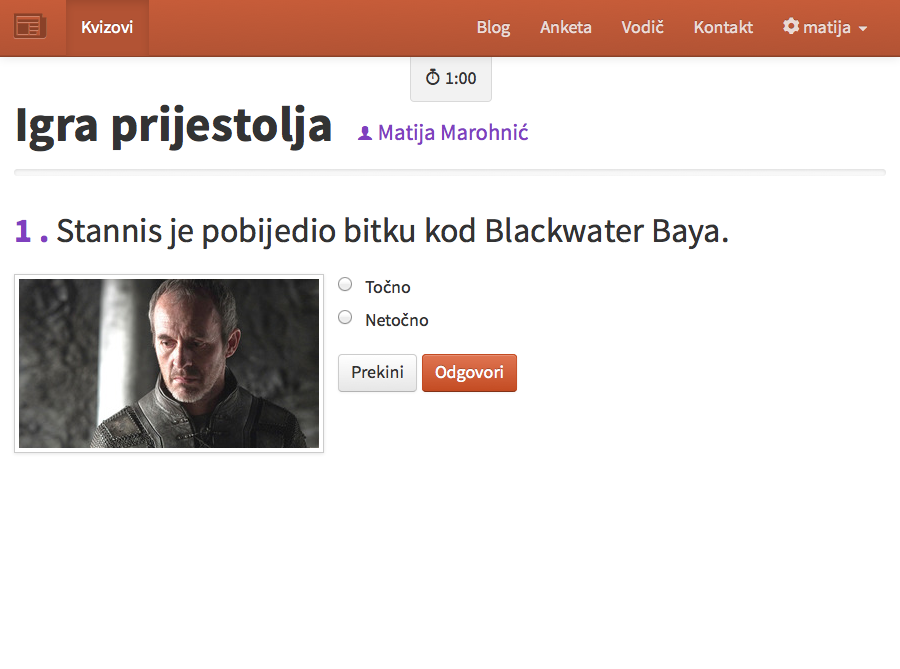
\includegraphics[width=\textwidth, clip=true, trim=0 7cm 0 0, fbox]{student/boolean_question}
  \caption{Pitanje vrste \emph{točno/netočno}}
  \label{fig:boolean}
\end{figure}

\subsection{Ponuđeni odgovori}

\emph{Ponuđeni odgovori} (slika \ref{fig:choice}) je vrsta pitanja gdje se
postavlja pitanje na koje treba odgovoriti \textbf{jednim} od ponuđenih
odgovora. Ova vrsta pitanja je teža od \emph{točno/netočno} jer se vjerojatnost
da korisnik točno odgovori smanjuje s brojem ponuđenih odgovora.

Razmišljali smo o tome da omogućimo više mogućih točnih odgovora, ali to bi
činilo ovu vrstu pitanja težom, pa smo odlučili odgoditi implementaciju te
značajke za jednu od budućih verzija aplikacije.

\begin{figure}[H]
  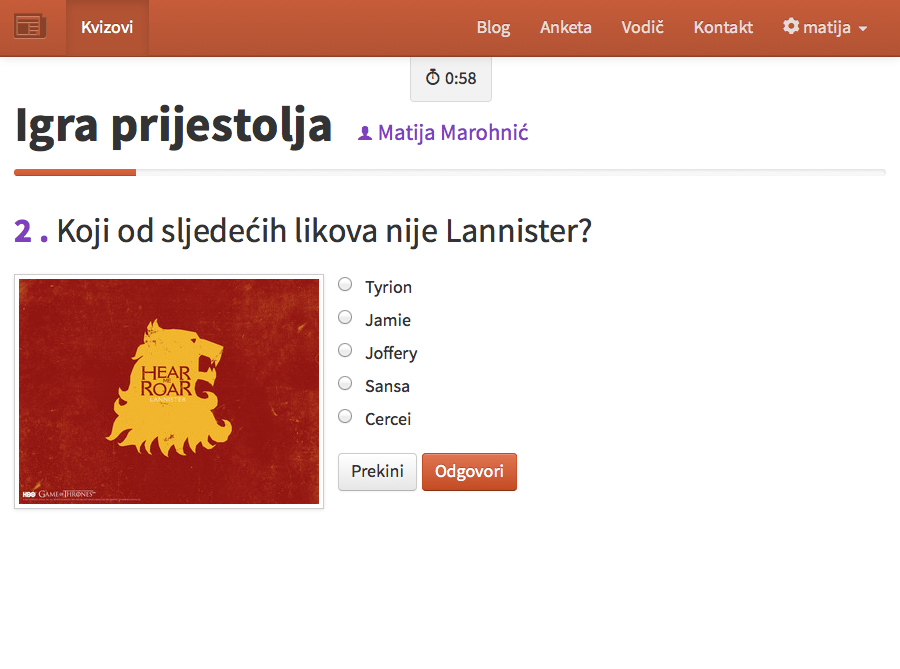
\includegraphics[width=\textwidth, clip=true, trim=0 5cm 0 0, fbox]{student/choice_question}
  \caption{Pitanje vrste \emph{ponuđeni odgovori}}
  \label{fig:choice}
\end{figure}

\subsection{Asocijacija}

\emph{Asocijacija} (slika \ref{fig:association}) je vrsta pitanja gdje korisnik
pridružuje pojmove iz jednog s pojmovima iz drugog stupca. Ovo pitanje je teže
od \emph{ponuđenih odgovora} jer se broj mogućih kombinacija eksponencijalno
povećava s brojem parova pojmova.

Ova vrsta pitanja bila je tehnički izazovna za dizajnirati jer postoji mnogo
različitih pristupa. Odlučili smo se za pristup gdje se pojmovi ``primaju'' s
mišem i ``ispuštaju'' na drugi pojam, nakon čega ta 2 pojma zamijenjuju mjesta.
Na taj način korisnik može preslagivati pojmove dok ne dobije željenu
kombinaciju.

\begin{figure}[H]
  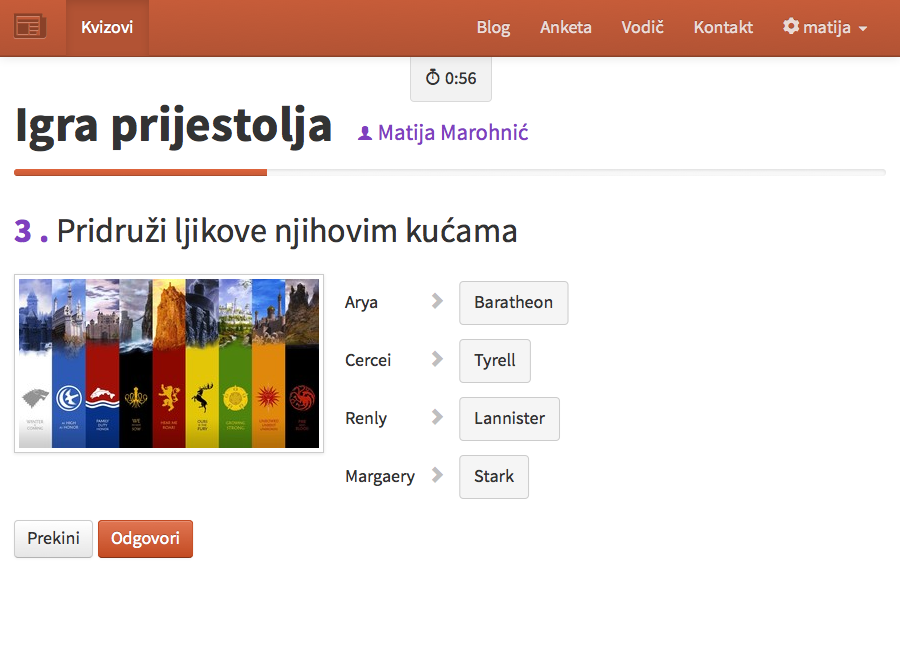
\includegraphics[width=\textwidth, clip=true, trim=0 3cm 0 0, fbox]{student/association_question}
  \caption{Pitanje vrste \emph{asocijacija}}
  \label{fig:association}
\end{figure}

\subsection{Upiši točan odgovor}

\emph{Upiši točan odgovor} (slika \ref{fig:text}) je vrsta pitanja gdje se
postavlja pitanje, a korisnik treba upisati točan odgovor u za to predviđeno
tekstualno polje. Ova vrsta pitanja je najteža zato što je vrlo lako pogriješiti
-- korisnik mora upisati odgovor točno onako kako ga je administrator napisao.

Kako bismo učinili ovu vrstu pitanja malo lakšom, dizajnirali smo ju tako da
nije bitno piše li korisnik malim ili velikim slovima, ako se slova podudaraju s
točnim odgovorom, dani se odgovor smatra točnim.

\begin{figure}[H]
  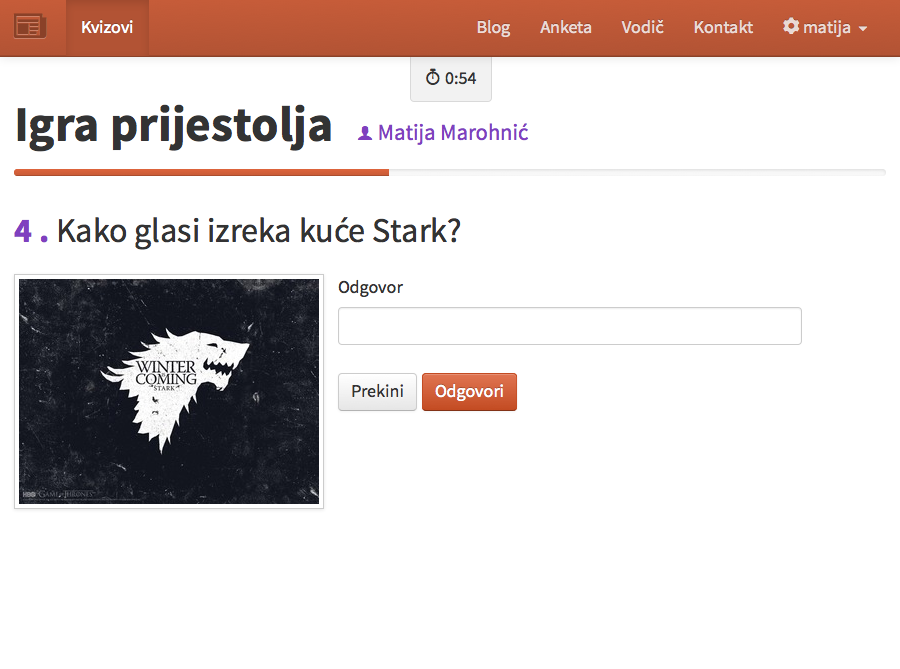
\includegraphics[width=\textwidth, clip=true, trim=0 5cm 0 0, fbox]{student/text_question}
  \caption{Pitanje vrste \emph{upiši točan odgovor}}
  \label{fig:text}
\end{figure}

\section{Izrada aplikacije}

\emph{Kvizovi} su web aplikacija, dakle koristi se pomoću web preglednika. Sa
strane klijenta (web preglednika) koristimo tehnologije kao što su HTML, CSS i
JavaScript, a sa strane poslužitelja koristimo programski jezik Ruby i
PostgreSQL relacijsku bazu. U narednim poglavljima ukratko opisujemo svaku od
tehnologija.

\subsection{Tehnologije na strani klijenta}

Ove tehnologije izvršavaju web preglednici, te su one jedinstvene, odnosno za
njih ne postoje alternative. Specifikacije ovih tehnologija razvija međunarodna
organizacija W3C (World Wide Web Consortium).

\subsubsection{HTML}

\begin{wrapfigure}{left}{2.5cm}
  \vspace{-10pt}
  
\includegraphics[width=2.5cm]{logos/html}
  \vspace{-30pt}
\end{wrapfigure}

HTML je jezik kojim se označava sadržaj i struktura web stranica, i sam po sebi
ne propisuje izgled, već web preglednik ima definirana CSS pravila za izgled
svakog HTML elementa u slučaju da web dizajner nije definirao svoja.\cite{html}

Za našu aplikaciju koristili smo najnoviju verziju HTML-a -- HTML5. Koristili
smo ju zbog novih funkcionalnosti koje pruža, kao što je povezivanje računala
što omogućuje nove značajke u aplikaciji kao što je grupno rješavanje kvizova.

\subsubsection{CSS}

\begin{wrapfigure}{right}{2.5cm}
  \vspace{-10pt}
  
\includegraphics[width=2.5cm]{logos/css}
  \vspace{-30pt}
\end{wrapfigure}

CSS je stilski jezik koji se koristi za opis prezentacije HTML dokumenata. Svaka
vrsta web preglednika ima drugačije implementiranu specifikaciju CSS-a, zbog
čega ga ponekad interpretira malo drugačije od ostalih preglednika. Zato je
izazovno napisati CSS na način da isto izgleda u svim web
preglednicima.\cite{css}

Za našu aplikaciju koristili smo najnoviju verziju CSS-a -- CSS3. Velik dio CSS3
specifikacije implementiran je u modernim web preglednicima, a u starijim se web
preglednicima izgled aplikacije mjestimično elegantno degradira, što ne utječe
negativno na njezinu funkcionalnost. Za pregledavanje podržanosti pojedinih CSS3
stilova u web preglednicima koristimo bazu podataka \url{caniuse.com}.

\subsubsection{JavaScript}

\begin{wrapfigure}{left}{2.5cm}
  \vspace{-10pt}
  
\includegraphics[width=2.5cm]{logos/javascript}
  \vspace{-30pt}
\end{wrapfigure}

JavaScript je skriptni programski jezik koji se koristi za dinamičku
manipulaciju HTML-a i komunikaciju sa poslužiteljem. Dok su drugi jezici obično
sintaktički funkcijski ili objektni, JavaScript se temelji na
prototipima.\cite{js}

U našoj aplikaciji koristili smo JavaScript kod odbrojavanje štoperice,
učitavanje slika za pitanja i drugih funkcionalnosti.

\subsection{Tehnologije na strani poslužitelja}

Ove tehnologije izvršavaju web poslužitelji. Za razliku od tehnologija na
strani klijenta, ove tehnologije imaju puno alternativa, a odabir određene
tehnologije je danas uglavnom subjektivan.

\subsubsection{Ruby}

\begin{wrapfigure}{right}{2.5cm}
  \vspace{-10pt}
  
\includegraphics[width=2cm]{logos/ruby}
  \vspace{-20pt}
\end{wrapfigure}

Ruby je višeplatformski jezik opće namjene i pripada klasi objektno-orjentiranih
jezika. Ruby je počeo biti jako popularan 2005. dolaskom
\emph{Rails}\footnote{\url{http://rubyonrails.org}} aplikacijskog okvira, u
kojemu smo razvili ovu aplikaciju.\cite{ruby}

Razlog zašto smo odabrali Ruby je zato što vrlo moćan i ima lijepu i čistu
sintaksu. Neke od popularnih alternativa uključuju: PHP, Python, C\#, Java itd.

\subsubsection{PostgreSQL}

\begin{wrapfigure}{left}{2.5cm}
  \vspace{-10pt}
  
\includegraphics[width=2.5cm]{logos/postgresql}
  \vspace{-30pt}
\end{wrapfigure}

PostgreSQL je sustav za upravljanje bazama podataka. U bazu podataka se spremaju
sve informacije koje trebaju biti trajne, poput informacija o
korisnicima.\cite{postgresql}

PostgreSQL je bio naš izbor zbog njegove količine funkcionalnosti i kvaliteti.
Neke od popularnih alternativa uključuju: MySQL, Microsoft SQL Server itd.

\subsection{Ostale tehnologije}

\subsubsection{Git i GitHub}

\begin{wrapfigure}{right}{2.5cm}
  \vspace{-10pt}
  
\includegraphics[width=2.5cm]{logos/git}
  \vspace{-30pt}
\end{wrapfigure}

Git je besplatan i otvoren distribuirani sustav za verzioniranje dizajniran da
upravlja svime od malih do jako velikih projekata s brzinom i
efikasnosti.\cite{git} Git nam je bio neizmjerno koristan u paralelnom pisanju
koda i samog rada.

\begin{wrapfigure}{left}{2.5cm}
  \vspace{-10pt}
  
\includegraphics[width=2.5cm]{logos/github}
  \vspace{-30pt}
\end{wrapfigure}

GitHub je web aplikacija koja omogućava učitavanje Git repozitorija (projekta)
te tako olakšava kolaboraciju među ljudima koji rade na projektu.\cite{github}
Neke od značajki GitHub-a su pregled promjena, mogućnosti za prijavljivanje
grešaka, listanje kôda itd.

\subsubsection{Gauges}

\begin{wrapfigure}{right}{2.5cm}
  \vspace{-10pt}
  
\includegraphics[width=2.5cm]{logos/gauges}
  \vspace{-30pt}
\end{wrapfigure}

Gauges je web aplikacija za pregled prometa web stranica u stvarnom vremenu.
Gauges pruža informacije kao broj pogleda, broj jedinstvenih posjetitelja,
države posjetitelja itd.\cite{gauges}

Gauges nam je vrlo pomogao u analizi posjetitelja, ponajviše zbog mogućnosti
uvida u to kakve web preglednike i koje uređaje su naši posjetitelji koristili
dok su posjećivali Kvizove.

\subsubsection{Heroku}

\begin{wrapfigure}{left}{2.5cm}
  \vspace{-10pt}
  
\includegraphics[width=2cm]{logos/heroku}
  \vspace{-30pt}
\end{wrapfigure}

Heroku je web servis koji pruža hosting web aplikacija u oblaku.\cite{heroku}
Uz Heroku nije potrebno konfigurirati poslužitelj na kojem se nalazi web
aplikacija, već to Heroku radi sam.

\section{Iz perspektive korisnika}

\subsection{Nastavnici}

\emph{Škola} je uloga koja predstavlja profesora i ona je administrator kvizova.

Nakon odabira te uloge korisnik se može prijaviti ili registrirati ako još nema
korisnički račun. Registracija se sastoji od ispunjavanja jednostavnog formulara
pomoću kojega skupljamo informacije o korisnicima koje možemo iskoristiti kako
bismo poboljšali njihovo iskustvo i kako bismo mogli raditi istraživanja. Polje
u formularu za registraciju na koje ćemo se osvrnuti je \emph{Tajni ključ}, koji
je potreban za registraciju učenicima te škole.

Nakon prijave, nastavnicima se otvara stranica s popisom kvizova koje su
kreirali (vidi sliku \ref{fig:school/quizzes}),

\begin{figure}[H]
  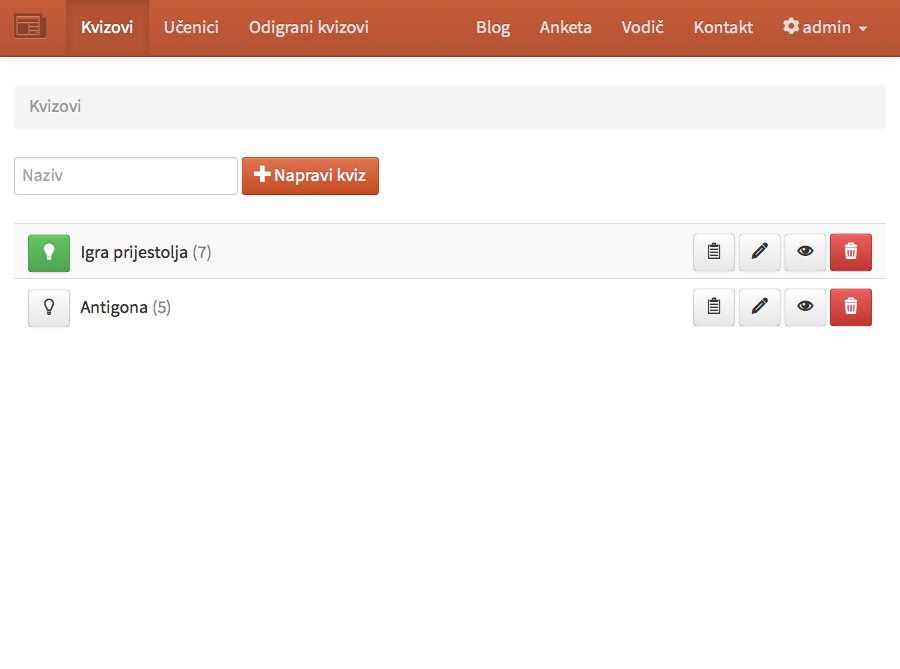
\includegraphics[width=\textwidth, clip=true, trim=0 10cm 0 0, fbox]{school/quizzes}
  \caption{Škole -- popis kvizova}
  \label{fig:school/quizzes}
\end{figure}

gdje mogu izmjenjivati postojeće kvizove i sastavljati nove. Nakon što je
profesor zadovoljan s kvizom, može ga učiniti aktivnim, odnosno vidljivim
učenicima. Izmjenjivanje kvizova podijeljeno je na izmjenu metapodataka kviza i
na izmjenu pitanja kviza. Ovdje napominjemo da ćemo, zbog zaštite privatnosti
naših korisnika, u radu prikazivati podatke kviza kojeg smo sami napravili
(Igra prijestolja), a našim imenima ćemo zamijeniti stvarna imena korisnika
koji su sudjelovali u istraživanju.

Uz svako se pitanje može pridružiti pomoć (slikom ili tekstom), koja će se
prikazati učenicima dok rješavaju pitanje.

Škole mogu pregledavati informacije o odigranim kvizovima: kada su igrani, tko
ih je igrao, koji su bili rezultati itd. (vidi \ref{played_quizzes} i \ref{played_quiz}).

\begin{figure}[H]
  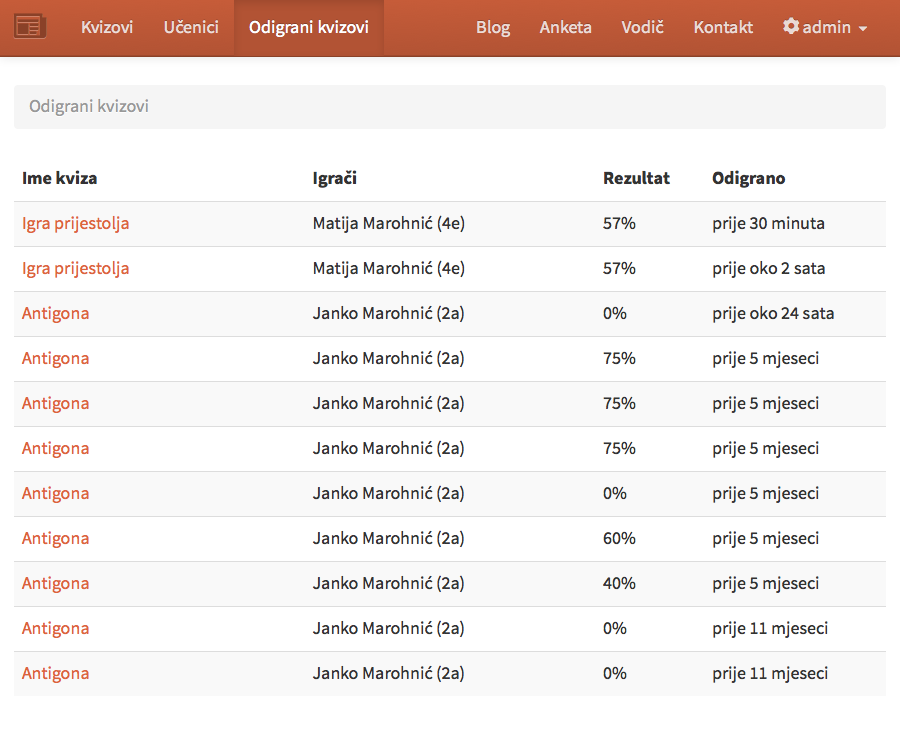
\includegraphics[width=\textwidth, clip=true, trim=0 10cm 0 0, fbox]{school/played_quizzes}
  \caption{Škole -- popis odigranih kvizova}
  \label{played_quizzes}
\end{figure}

\begin{figure}[H]
  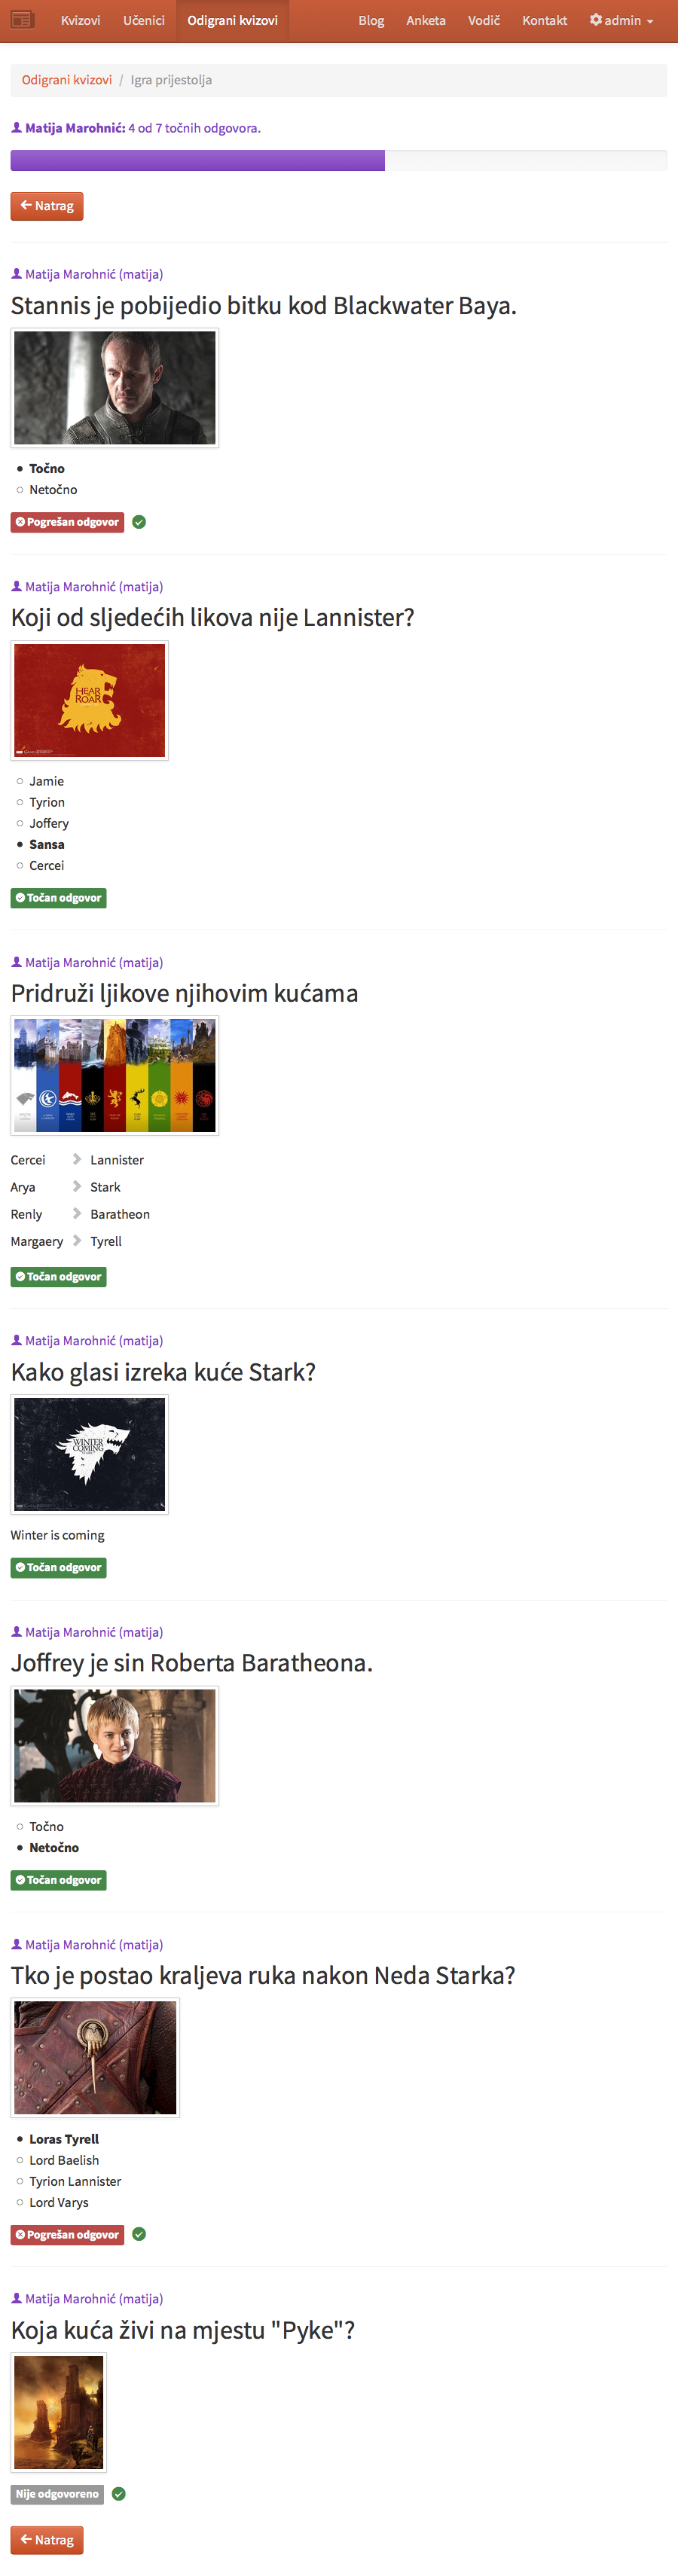
\includegraphics[width=\textwidth, clip=true, trim=0 80cm 0 0, fbox]{school/played_quiz}
  \caption{Odigrani kviz}
  \label{played_quiz}
\end{figure}

Mogu se pregledavati i učenici, koliko su kvizova odigrali, koji su to kvizovi i
sl. (vidi sliku \ref{students}).

\begin{figure}[H]
  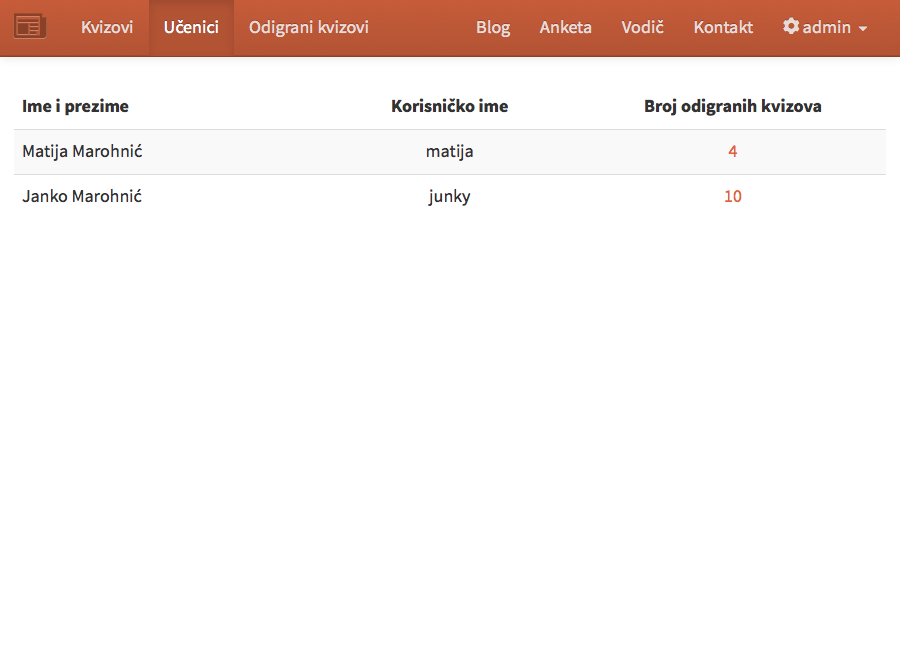
\includegraphics[width=\textwidth, clip=true, trim=0 15cm 0 0, fbox]{school/students}
  \caption{Škole -- popis učenika}
  \label{students}
\end{figure}

\subsection{Učenici}

\emph{Učenik} je uloga koja rješava kvizove koje je napravila njihova škola. Kao
i kod škole, učenik se može prijaviti ili registrirati, ako već nema korisnički
račun. Pri registraciji učenik treba napisati tajni ključ koji mu je njegova
škola dala, u protivnom se ne može registrirati. Na taj način sprječavamo da se
bilo tko registrira kao učenik.

Nakon prijave ili registracije, korisnika dočeka lista kvizova koji su dostupni
za rješavanje. Kviz je moguće igrati samostalno ali i u paru (vidi sliku
\ref{student/quizzes}). U drugom slučaju, drugi igrač također mora biti prijavljen
u sustav.

\begin{figure}[H]
  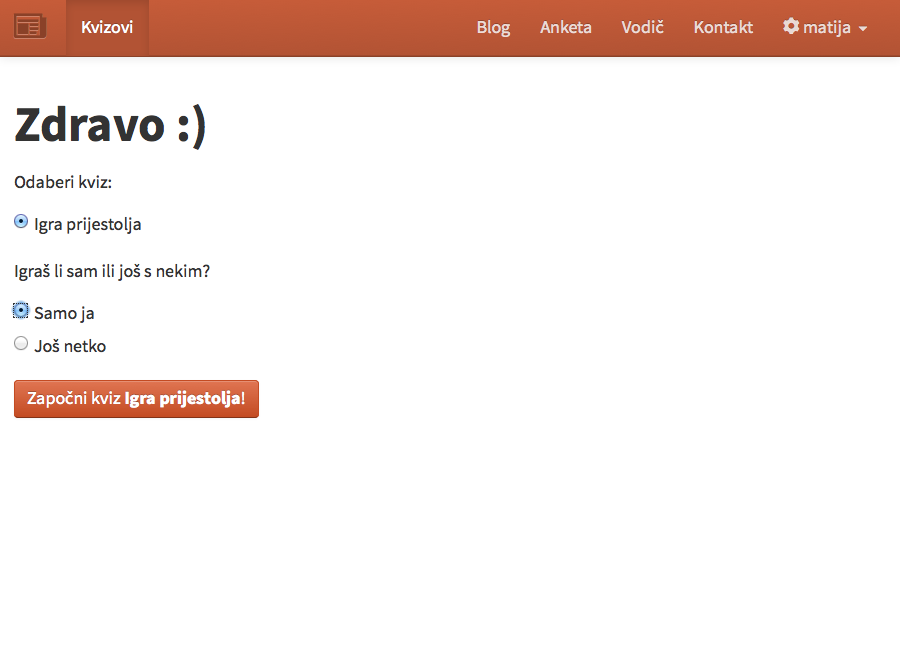
\includegraphics[width=\textwidth, clip=true, trim=0 8.5cm 0 0, fbox]{student/quizzes}
  \caption{Učenici -- popis kvizova}
  \label{student/quizzes}
\end{figure}

Nakon što učenik započne kviz, prikazuje mu se jedno po jedno pitanje na koja
treba odgovoriti. Kako bi igra bila što poštenija, pitanja su obično vremenski
ograničena, tako da se učenik ne stigne previše konzultirati s vanjskim
izvorima. Preostalo vrijeme ispisano je iznad imena korisnika (vidi sliku
\ref{question}).

\begin{figure}[H]
  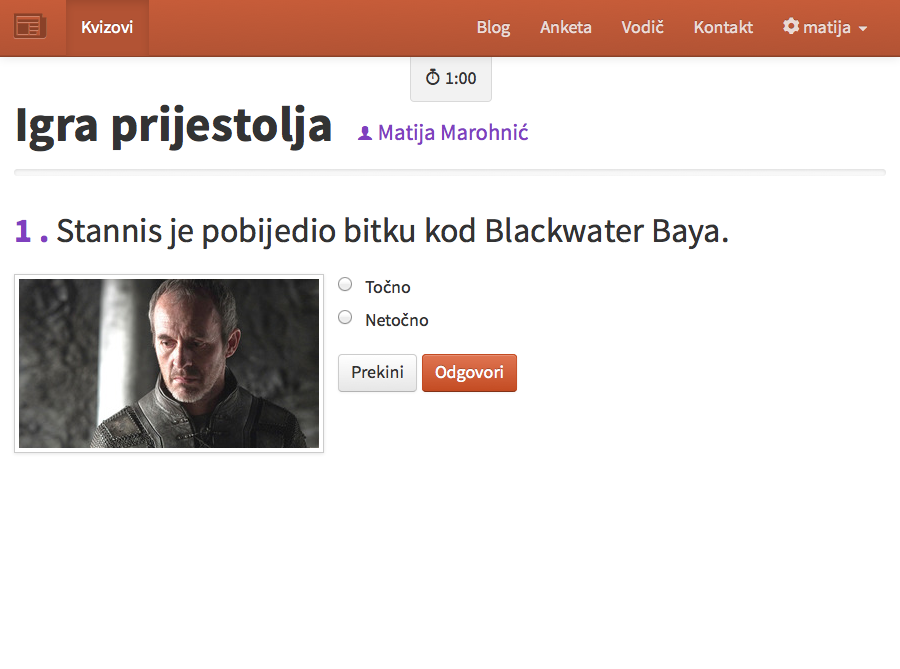
\includegraphics[width=\textwidth, clip=true, trim=0 7cm 0 0, fbox]{student/boolean_question}
  \caption{Učenici -- odgovaranje na pitanje}
  \label{question}
\end{figure}

\begin{figure}[H]
  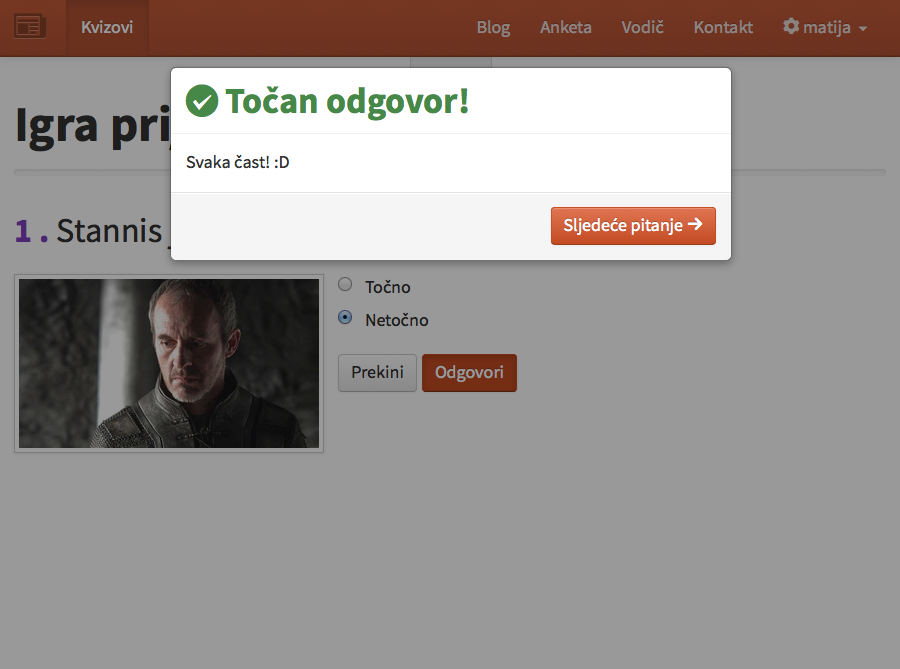
\includegraphics[width=\textwidth, clip=true, trim=0 7cm 0 0, fbox]{student/boolean_question_correct}
  \caption{Učenici -- povratna informacija nakon predanog odgovora}
\end{figure}

Nakon što učenik odgovori na sva pitanja, ispisuju se rezultati i učenik dobiva
određenu ``titulu'' s obzirom na njegov rezultat:

\begin{description}
  \item[Znalac-malac] 0\%-30\% točnih odgovora
  \item[Ekspert] 30\%-70\% točnih odgovora
  \item[Super-ekspert] 70\%-100\% točnih odgovora
\end{description}

Titule su osmišljene zato da se učenika uvijek pohvaljuje, čak i ako je imao loš
rezultat, tako da se učenik dobro osjeća i da ga se potiče da igra i dalje.

\chapter{Rezultati}
\label{chap:results}

Istraživanje smo proveli tako što smo izradili aplikaciju za kvizove (vremenski
period od početka izrade do završetka prve verzije: 9.7-22.8.2012.) i dali
određenom uzorku osnovnih i srednjih škola na testiranje. Do danas je
registrirano 20 škola i 401 učenik.

U svakom razredu su učenici bili podijeljeni na skupinu koja ne rješava kvizove
i na onu koja rješava. Na taj način smo mogli provjeravati učinkovitost
aplikacije kada bi učenici imali test znanja. Iako smo prikupili dosta podataka
o korištenju aplikacije, na 16.03.2013. smo proveli i anketu među nastavnicima
ali i učenicima kako bismo dobili neke dodatne informacije koje na drugi način
nismo mogli dobiti. Na anketu je odgovorilo sveukupno 5 škola i 30 učenika.
Budući da je anketa prevelika, ne možemo je uključiti u prilog, ali u sljedećim
slikama prikazujemo rezultate najvažnijih pitanja.

\section{Škole}

Ankete su pokazale da je većina profesora primijetila napredak u
poznavanju gradiva kod svojih učenika, kao i veću zainteresiranost za gradivo
(vidi slike \ref{fig:school/advance}, \ref{fig:school/comparison} i
\ref{fig:school/help}).

\begin{figure}[H]
  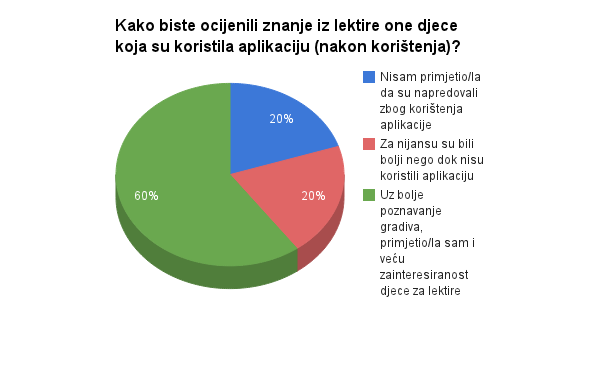
\includegraphics[width=\textwidth, clip=true, trim=0 2.5cm 0 0]{school/advance}
  \caption{Napredak učenika}
  \label{fig:school/advance}
\end{figure}

\begin{figure}[H]
  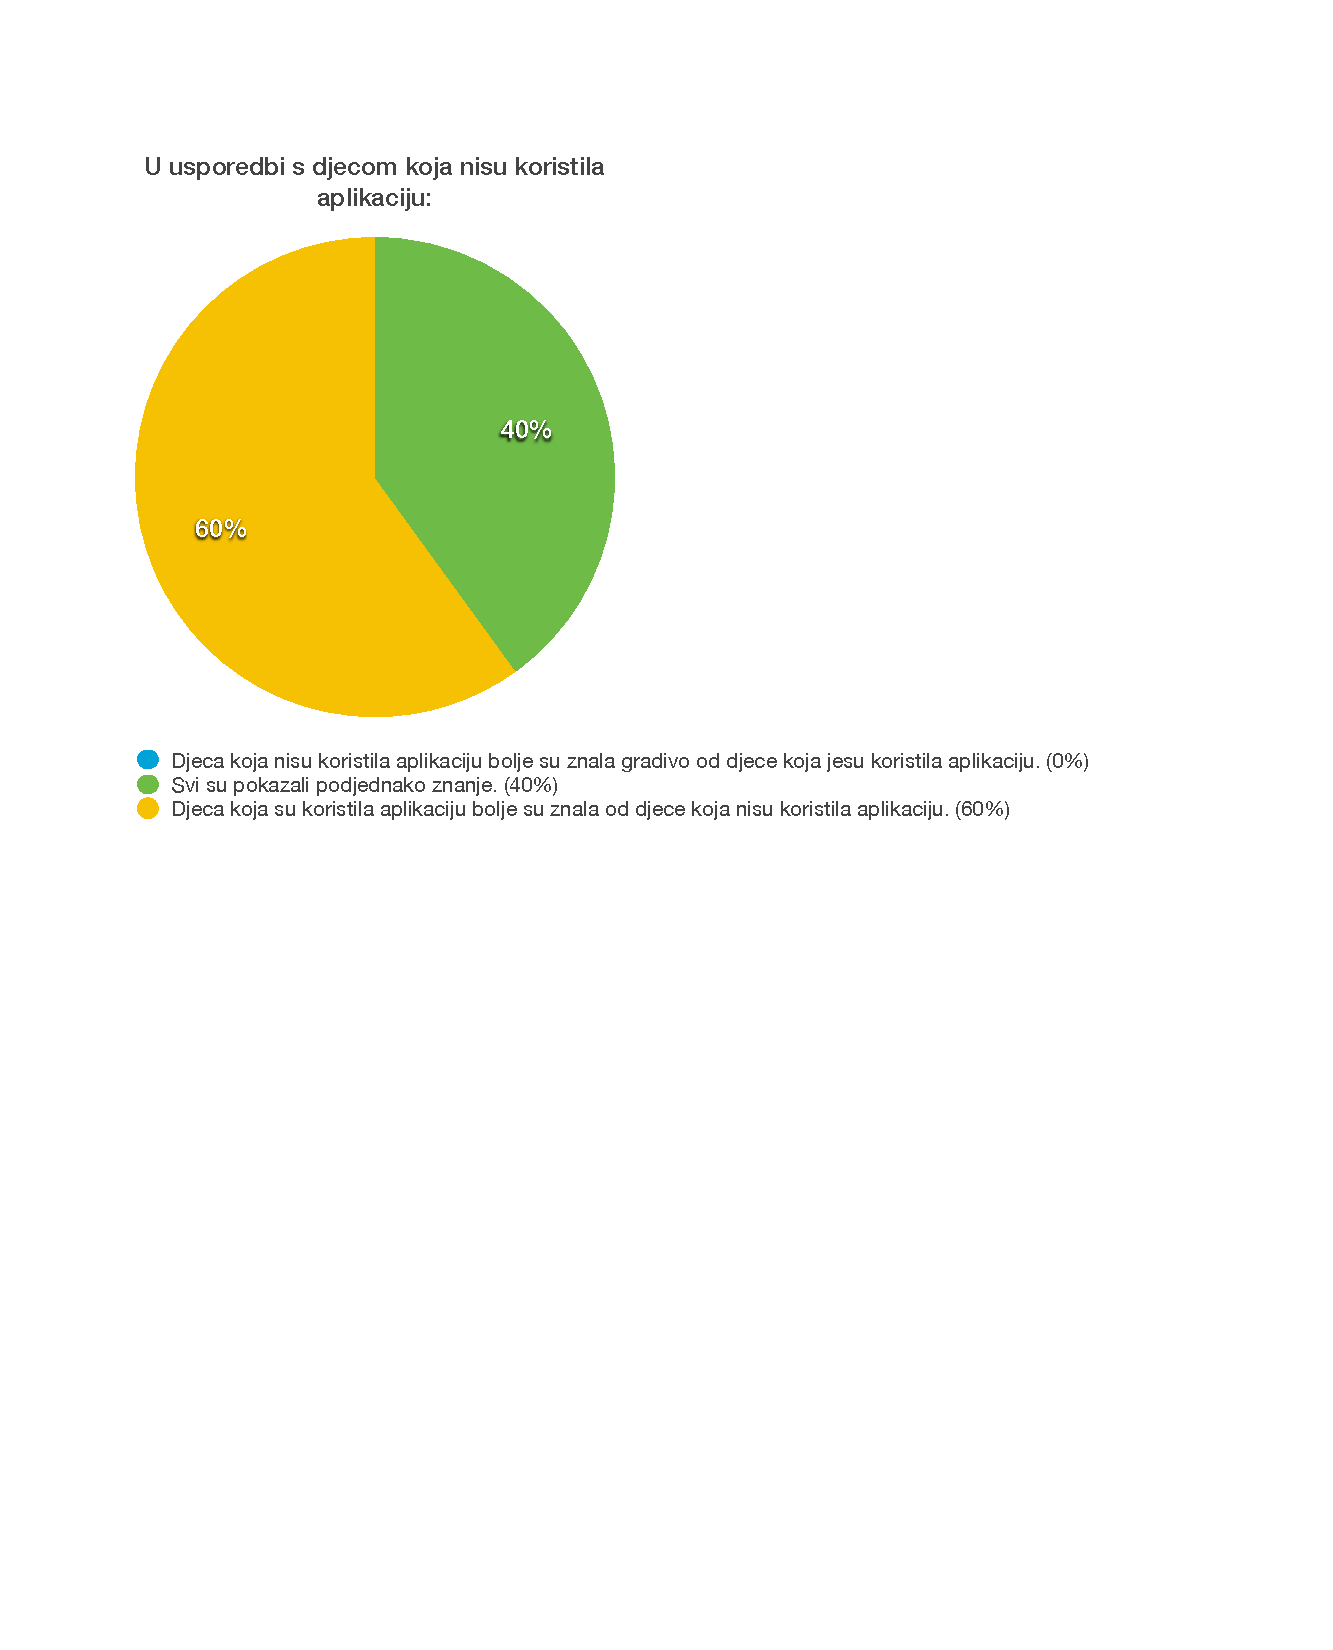
\includegraphics[width=\textwidth, clip=true, trim=0 2.5cm 0 0]{school/comparison}
  \caption{Usporedba učenika koji su koristili aplikaciju s onima koji nisu}
  \label{fig:school/comparison}
\end{figure}

\begin{figure}[H]
  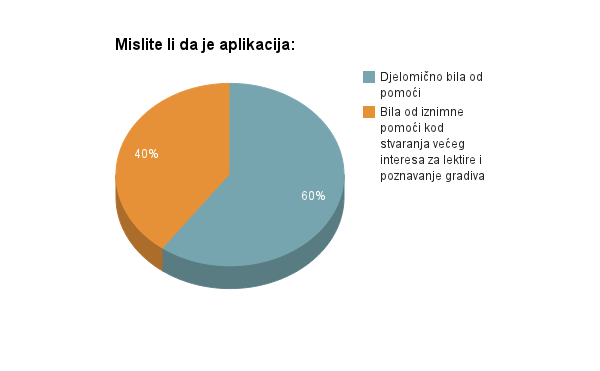
\includegraphics[width=\textwidth, clip=true, trim=0 2.5cm 0 0]{school/help}
  \caption{Poticanje interesa učenika za gradivo}
  \label{fig:school/help}
\end{figure}

\section{Učenici}

Kod učenika su ankete pokazale da učenici smatraju ovakav način učenja
učinkovitim (vidi slike \ref{fig:student/interesting},
\ref{fig:student/effective} i \ref{fig:student/help}).

S druge strane, pokazalo je tek pola učenika osjetilo poboljšanje u ocjeni
(vidi sliku \ref{fig:student/grades}).

\begin{figure}[H]
  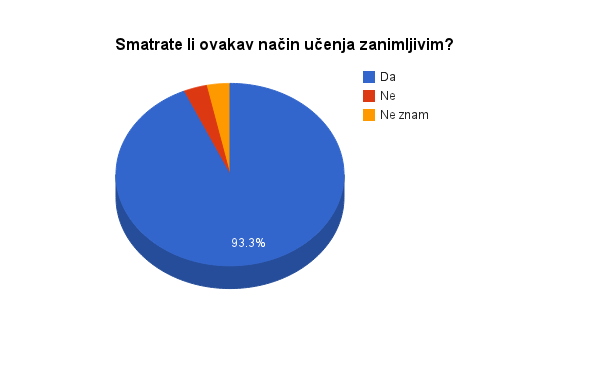
\includegraphics[width=\textwidth, clip=true, trim=0 2.5cm 0 0]{student/interesting}
  \caption{Zanimljivost učenicima}
  \label{fig:student/interesting}
\end{figure}

\begin{figure}[H]
  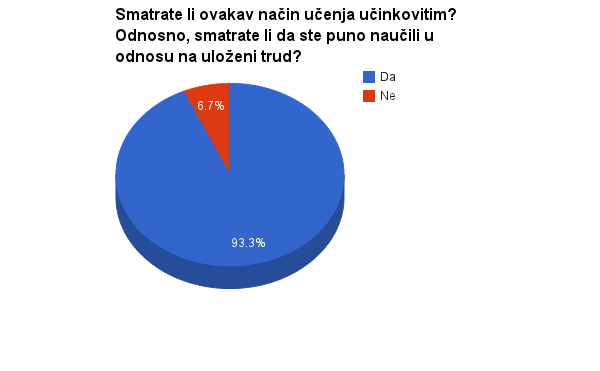
\includegraphics[width=\textwidth, clip=true, trim=0 2.5cm 0 0]{student/effective}
  \caption{Učinkovitost učenicima}
  \label{fig:student/effective}
\end{figure}

\begin{figure}[H]
  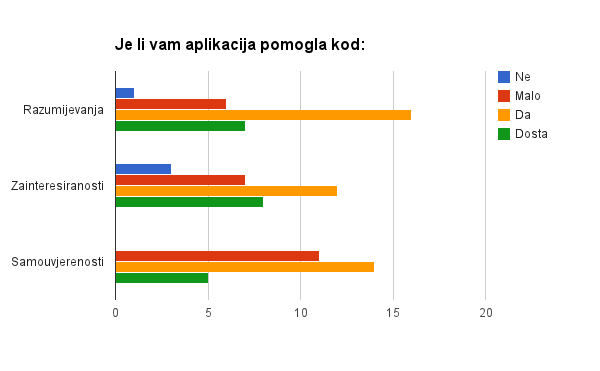
\includegraphics[width=\textwidth, clip=true, trim=0 2.5cm 0 0]{student/help}
  \caption{Pomoć učenicima pri razumijevanju, zainteresiranosti i samouvjerenosti}
  \label{fig:student/help}
\end{figure}

\begin{figure}[H]
  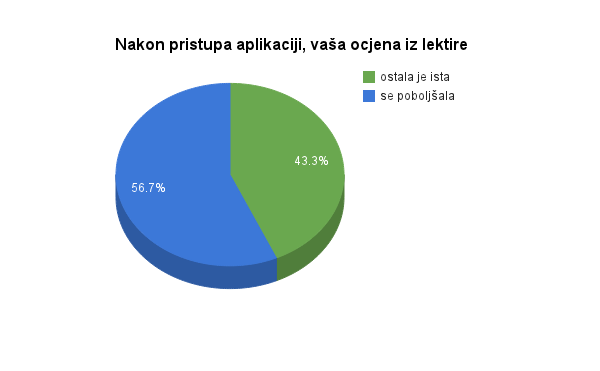
\includegraphics[width=\textwidth, clip=true, trim=0 2.5cm 0 0]{student/grades}
  \caption{Promjena ocjene kod učenika}
  \label{fig:student/grades}
\end{figure}

\chapter{Zaključak}

Profesori su primjetili napredak kod učenika koji su koristili aplikaciju u
odnosu na one koji nisu i sami su učenici osjetili poboljšanje na više razina,
ali samo su se polovici učenika koji su koristili aplikaciju poboljšale ocijene
iz lektire. S obzirom da aplikacija još nije gotova, možda će se taj omjer
promijeniti na bolje s vremenom.

Osim zbog interaktivnosti, ovakav način podučavanja dobro funkcionira zato što
možemo na licu mjesta ispravljati greške i ažurirati aplikaciju prema povratnim
informacijama dok ju učenici i profesori koriste. Ovakav se način podučavanja
može puno brže mijenjati od mnogih tradicionalnih načina podučavanja kao što su
testovi, profesori mogu prepraviti kvizove u aplikaciji čim uoče grešku i te će
promjene odmah stupiti na snagu, a da ih učenici neće ni primjetiti.

Radimo na tome da sučelje aplikacije bude dovoljno jednostavno da vodič za
aplikaciju više neće biti potreban, već da je jasno samo po sebi kako postići
određeni cilj. Iako aplikaciju koriste stariji profesori koji nisu vješti u
korištenju aplikacije, vjerujemo da korisnici više vole učiti kako koristiti
aplikaciju iz prakse, a ne čitajući upute i da aplikaciju možemo učinit dovoljno
jednostavnom da je pristupačna za svaki uzrast i stupanj informatičke
obrazovanosti.

Aplikacija \emph{Kvizovi} je inicijalno nastala kao pomoćno sredstvo za učenje
lektira, ali s obzirom na pozitivan utjecaj na učenike i profesore i rezultatima
iz anketa više ne vidimo razlog zašto se aplikacija ne bi koristila i za ostale
školske predmete kao što su zemljopis, biologija, kemija itd.

\chapter{Zahvale}

Htjeli bismo zahvaliti našoj mentorici, doc. dr. sc. Kristini Kocijan na ideji
aplikacije \emph{Kvizovi}, strukturiranju ovoga rada, na prikupljanju uzorka
škola koje su bile voljne koristiti našu aplikaciju i velikom strpljenju tijekom
ove 2 godine. Također, zahvaljujemo se kolegici Marti Mihaljević na lektoriranju
ovoga rada. Nadalje, htjeli bismo zahvaliti profesorima i učenicima iz ispitanog
uzorka na sudjelovanju u ovom istraživanju i na slanju prijedloga i prijavu
grešaka, što nam je puno pomoglo u razvijanju aplikacije.

Sortirane prema broju aktivnih kvizova, škole koje su sudjelovale u istraživanju
su: I. gimnazija, Osnovna škola Bogumila Tonija, Osnovna škola Stjepana Radića,
Srednja škola Metković, Osnovna škola Poreč, Osnovna škola Stubičke Toplice,
Gimnazija Sesvete, Poljoprivredna škola, Srednja škola ``Ivan Seljanec''
Križevci, Gimnazija fra Dominika Mandica, Medicinska škola Varaždin, Srednja
škola Čakovec, Tehnička škola Šibenik, Privatna srednja ekonomska škola INOVA,
Škola za umjetnost, dizajn, grafiku i odjeću, Zabok, Gimnazija i strukovna
škola Jurja Dobrile, Nadbiskupska klasična gimnazija.

\renewcommand{\listoffigures}{\begingroup
\tocchapter
\tocfile{\listfigurename}{lof}
\endgroup}

\listoffigures

\renewcommand{\bibname}{Popis literature}

\begin{thebibliography}{99}

  \raggedright

  \bibitem{perisic13} Perišić, Kristina. “Kako poboljšati koncentraciju djeteta?”
    Klokanica.hr, May 21, 2013.
    \url{http://www.klokanica.hr/skolarci/skola/kako-poboljsati-koncentraciju-djeteta-168}.

  \bibitem{clark11} Clark, Donald. “Visual, Auditory, and Kinesthetic Learning
    Styles (VAK).” The Performance Juxtaposition, December 7, 2011.
    \url{http://www.nwlink.com/~donclark/hrd/styles/vakt.html}.

  \bibitem{html} “HTML.” Wikipedija, April 20, 2014.
    \url{http://hr.wikipedia.org/w/index.php?title=HTML&oldid=4285227}.

  \bibitem{css} “CSS.” Wikipedija, April 15, 2014.
    \url{https://hr.wikipedia.org/w/index.php?title=CSS&oldid=4154816}.

  \bibitem{js} “JavaScript.” Wikipedija, April 24, 2014.
    \url{https://hr.wikipedia.org/w/index.php?title=JavaScript&oldid=3942542}.

  \bibitem{w3c} “World Wide Web Consortium (W3C).” W3C, April 25, 2014.
    \url{http://www.w3.org}.

  \bibitem{git} GitHub, Inc. “Git.” Git, April 28, 2014.
    \url{http://git-scm.com}.

  \bibitem{gauges} GitHub, Inc. “Gauges.” Real Time Analytics Service | Gauges,
    April 28, 2014. \url{http://get.gaug.es/}.

  \bibitem{github} GitHub, Inc. “GitHub · Build Software Better, Together.”
    GitHub, April 28, 2014. \url{https://github.com/}.

  \bibitem{mit} GitHub, Inc. “MIT License - ChooseALicense.com.”
    ChooseALicense.com, February 16, 2014.
    \url{http://choosealicense.com/licenses/mit/}.

  \bibitem{ruby} “Ruby Programming Language.” Ruby, April 27, 2014.
    \url{https://www.ruby-lang.org/en/}.

  \bibitem{postgresql} “PostgreSQL: The World’s Most Advanced Open Source
    Database.” PostgreSQL, April 28, 2014. \url{http://www.postgresql.org/}.

  \bibitem{heroku} "Heroku | Cloud Application Platform." Heroku, April 29,
    2014. \url{https://www.heroku.com/}

  \bibitem{krug05} Krug, Steve. Don’t Make Me Think! : A Common Sense Approach
    to Web Usability. 2nd edition. Berkeley, California USA: New Riders, 2005.

  \bibitem{kvizovinet} “Kvizovi.net :: Znanje je sexy ;-).” Kvizovi.net, April
    28, 2014. \url{http://kvizovi.net/}.

  \bibitem{kvizoteka} “kvizovi | kvizovi znanja | kviz igre | nagradni kvizovi |
    KVIZOTEKA.” Kvizoteka, April 28, 2014. \url{http://www.kvizoteka.net/}.

  \bibitem{ucionica} Wargog. “Ucionica on the App Store on iTunes.” iTunes,
    April 28, 2014.
    \url{https://itunes.apple.com/hr/app/ucionica/id566902215?mt=8}.

  \bibitem{quizup} Plain Vanilla Corp. “QuizUp™ on the App Store on iTunes.”
    iTunes, April 28, 2014.
    \url{https://itunes.apple.com/hr/app/quizup/id718421443?mt=8}.

\end{thebibliography}

\chapter{Sažetak}

\textbf{Ključne riječi}:

\chapter{Summary}

\textbf{Keywords}:

\end{document}
